\documentclass[a4paper]{ltxdoc}
\usepackage{lmodern}			% Usa a fonte Latin Modern			
\usepackage[T1]{fontenc}		% seleção de códigos de fonte.
\usepackage[utf8]{inputenc}		% determina a codificação utiizada (conversão automática dos acentos)
\usepackage{hyperref}  			% controla a formação do índice
\usepackage{parskip}			% espaçamento entre os parágrafos
\usepackage{microtype} 			% para melhorias de justificação
\usepackage{morefloats}			% permite mais floats
\usepackage[absolute]{textpos}
\usepackage{tabularx}
\usepackage[table]{xcolor}
\usepackage{graphicx}
\usepackage{mathtools}
\usepackage{multirow}

% Babel e ajustes
\usepackage[english,brazil]{babel}		% idiomas
\addto\captionsbrazil{
  %% ajusta nomes padroes do babel
  \renewcommand{\bibname}{Refer\^encias}
  \renewcommand{\indexname}{\'Indice}
  \renewcommand{\listfigurename}{Lista de ilustra\c{c}\~{o}es}
  \renewcommand{\listtablename}{Lista de tabelas}
  %% ajusta nomes usados com a macro \autoref
  \renewcommand{\pageautorefname}{p\'agina}
  \renewcommand{\sectionautorefname}{se{\c c}\~ao}
  \renewcommand{\subsectionautorefname}{subse{\c c}\~ao}
  \renewcommand{\paragraphautorefname}{par\'agrafo}
  \renewcommand{\subsubsectionautorefname}{subse{\c c}\~ao}
  \renewcommand{\paragraphautorefname}{subse{\c c}\~ao}
}  

\usepackage{color}
\definecolor{thered}{rgb}{0.65,0.04,0.07}
\definecolor{thegreen}{rgb}{0.06,0.44,0.08}
\definecolor{thegrey}{gray}{0.5}
\definecolor{theshade}{rgb}{1,1,0.97}
\definecolor{theframe}{gray}{0.6}
\definecolor{blue}{RGB}{41,5,195}
\newcommand{\orientador}{Prof. Dr. Pedro Paulo Balbi de Oliveira}
\newcommand\tab[1][1cm]{\hspace*{#1}}
\IfFileExists{listings.sty}{
  \usepackage{listings}
  \lstset{%
    language=[LaTeX]TeX,
    columns=flexible,
    basicstyle=\ttfamily\small,
    backgroundcolor=\color{theshade},
    frame=single,
    tabsize=2,
    rulecolor=\color{theframe},
    title=\lstname,
    escapeinside={\%*}{*)},
    breaklines=true,
    commentstyle=\color{thegrey},
    keywords=[0]{\fichacatalografica,\errata,\folhadeaprovacao,\dedicatoria,\agradecimentos,\epigrafe,\resumo,\siglas,\simbolos,\citacao,\alineas,\subalineas,\incisos},
    keywordstyle=[0]\color{thered},
    keywords=[1]{},
    keywordstyle=[1]\color{thegreen},
    breakatwhitespace=true,
    alsoother={0123456789_},
    inputencoding=utf8,
    extendedchars=true,
    literate={á}{{\'a}}1 {ã}{{\~a}}1 {é}{{\'e}}1 {è}{{\`{e}}}1 {ê}{{\^{e}}}1 {ë}{{\¨{e}}}1 {É}{{\'{E}}}1 {Ê}{{\^{E}}}1 {û}{{\^{u}}}1 {ú}{{\'{u}}}1 {â}{{\^{a}}}1 {à}{{\`{a}}}1 {á}{{\'{a}}}1 {ã}{{\~{a}}}1 {Á}{{\'{A}}}1 {Â}{{\^{A}}}1 {Ã}{{\~{A}}}1 {ç}{{\c{c}}}1 {Ç}{{\c{C}}}1 {õ}{{\~{o}}}1 {ó}{{\'{o}}}1 {ô}{{\^{o}}}1 {Õ}{{\~{O}}}1 {Ó}{{\'{O}}}1 {Ô}{{\^{O}}}1 {î}{{\^{i}}}1 {Î}{{\^{I}}}1 {í}{{\'{i}}}1 {Í}{{\~{Í}}}1,
  }
  \let\verbatim\relax
  \lstnewenvironment{verbatim}[1][]{\lstset{##1}}{}
}

\usepackage[alf]{abntex2cite}	% citacoes

\newcommand{\abnTeXSite}{}

\title{\protect\parbox{\textwidth}{\protect\centering \textbf{Conservabilidade de estados de autômatos celulares elementares com atualizações assíncronas por prioridade da vizinhança}}}

\author{Marcelo Vironda Rozanti\\\abnTeXSite Felipe Stefanelli de Aguiar Silva\\\abnTeXSite} 

\date{\today}

\hypersetup{
  pdftitle={Conservabilidade de estados de autômatos celulares elementares com atualizações assíncronas por prioridade da vizinhança},
  pdfauthor={Marcelo Vironda Rozanti}{Felipe Stefanelli de Aguiar Silva},
  pdfkeywords={Asynchronous priority based updating, Elementary Cellular Automata, New Kind of Science, Discrete dynamical systems, Number-conserving}, 
  pdfproducer={Marcelo Vironda Rozanti},
  pdfcreator={vim+LaTeX+abnTeX2},
  colorlinks=true,
  linkcolor=black,
  citecolor=black,
  urlcolor=blue
}

% \EnableCrossrefs
\CodelineIndex
% \RecordChanges
\hyphenpenalty=1000

\begin{document}

\thispagestyle{empty}
\huge{\centerline{UNIVERSIDADE PRESBITERIANA MACKENZIE}}

\bigskip
\bigskip

\centerline{\large{FACULDADE DE COMPUTAÇÃO E INFORMÁTICA}}

\makeatletter
\vfill
\large{\centering{\@author}}

\vspace*{\fill}

\large{Conservabilidade de estados de autômatos celulares elementares com}
\large{\centerline{atualizações assíncronas por prioridade da vizinhança}}

\vspace*{\fill}
\large{\centerline{SÃO PAULO}}
\large{\centerline{2019}}

\pagebreak

\large{\centering{\@author}}
\vfill
\large{\centerline{\@title}}
\vfill
\vspace*{\fill}

Orientador: \orientador
\\
\\
\\


\large{\centerline{SÃO PAULO}}
\large{\centerline{2019}}

\begin{textblock}{6}(9,9)
  % Projeto do Trabalho de Conclusão de Curso apresentado à Faculdade de Computação e Informática da Universidade Presbiteriana, desenvolvida como requisito parcial para aprovação na disciplina de Metodologia da Pesquisa em Computação, ministrada pelo professor Dr. Everton Knihs, do curso de Ciência da Computação.
\end{textblock}

\maketitle

\begin{abstract}
  Autômatos Celulares são sistemas computacionais discretos que se têm provado úteis como modelos genéricos de complexidade e representação de diversas dinâmicas em uma varidade de áreas científicas. Estes sistemas podem ser especificados puramente em termos matemáticos e até implementados em estruturas físicas. Muitos deles podem computar funções e resolver problemas algorítmicos. O presente projeto explora um conjunto fundamental deles, chamados Automatos Celulares Elementares com um tipo específico de atualização assíncrona baseada em prioridade da vizinhança com a esperança de encontrar modelos que podem ser usados em aplicações práticas onde há ambientes dinâmicos que apresentam conservabilidade. 
  % O código correspondende a este trabalho pode ser acessado no repositório \url{https://github.com/mvrozanti/TCC}.
\end{abstract}
Palavras-chave: Autômatos celulares elementares, atualização assíncrona por prioridade da vizinhança, New Kind of Science, Sistemas dinâmicos discretos, Conservabilidade

\vfill

\selectlanguage{english}
\begin{abstract}
  Cellular Automata are discrete computational systems that have proved useful as general models of complexity and representations of dynamics on a variety of scientific fields. These systems can be specified in purely mathematical terms and be implemented in physical structures. Many of them can compute functions and solve algorithmic problems. The present project attempts to explore a fundamental subset of them, called Elementary Cellular Automata with a specific kind of neighbourhood-priority-based asynchronous updating in the search of number-conserving models, which can be used for a variety of practical applications. 
  %The implementation developed is hosted at \url{https://github.com/mvrozanti/TCC}.
\end{abstract}
Keywords: \@pdfkeywords

\break

\selectlanguage{brazil}
\renewcommand{\contentsname}{\centerline{\Large Sumário}}

\tableofcontents

\listoftables

\listoffigures

\break

\section{INTRODUÇÃO}

% \tab Este projeto teve como objetivo explorar propriedades conservativas em autômatos celulares (ACs) elementares com atualização assíncrona baseada em prioridade da vizinhança. 

\tab Autômatos Celulares (ACs) são uma categoria de sistemas discretos. Por sua própria simplicidade, estes sistemas têm ocupado uma posição privilegiada no estudo de complexidade nos mais diversos campos da ciência, de biologia teórica a economia, entre muitos outros. O desenvolvimento de ACs é tipicamente atribuído a John von Neumann através de suas tentativas de desenvolver um modelo abstrato de autoreprodução biológica. Ao fim de 1950, foi notado que ACs poderiam ser vistos como computadores paralelos \cite[p. 876]{wolfram2002new}. Apesar de falta de investigação científica até 1970, um exemplo de AC se tornou muito famoso por seu comportamento complexo e regras simplesmente descritas inventadas por John Conway, \textit{The Game of Life}, que se popularizou após sua aparição na revista \textit{Scientific American}. 

\tab Desde então, múltiplos estudos compreensivos foram realizados por cientistas ao redor do mundo, destacando os trabalhos feitos por Stephen Wolfram na década de 1980, culminando na publicação do livro A New Kind of Science em que Wolfram apresenta uma coleção de resultados a respeito de ACs, com uma série de descobertas revolucionárias. 

% \tab No capítulo \ref{referencial}, é apresentado alguns conceitos básicos referentes à definição dos ACs. 

\subsection{CONTEXTUALIZAÇÃO E RELEVÂNCIA} \label{contex}

\tab A motivação inicial para o estudo de ACs por parte de von Neumann não era matemática mas tinha como diretriz encontrar uma forma viável de tratar do problema de como fazer máquinas se reproduzirem. Hoje é sabido que esses sistemas são aplicáveis para resolver problemas relativos a classificação de densidade, simulação de partículas, compressão de dados, design estrutural, representação de comportamentos dinâmicos como trânsito em cidades ou movimentação de seres vivos entre muitos outros.

\tab Há uma infinitude de ACs possíveis de serem engenhados. Um problema de possível realização através de ACs com propriedades conservativas, como é notado por \citeonline[p. 3]{yuen2009applications}, é na modelagem de trânsito de veículos: ``Uma abordagem para reduzir o congestionamento seria construir estradas novas ou ampliar as existentes para fornecer faixas adicionais e consequentemente, aumentar a capacidade da infraestrutura rodoviária. No entanto, essa abordagem pode ser muito custosa e os atrasos podem piorar enquanto as obras rodoviárias estão em andamento. Às vezes é difícil melhorar a estrada existente devido a objetivos ambientais ou sociais. Outra abordagem pode ser controlar o tráfego de tal maneira que o congestionamento seja resolvido com o uso de semáforos ou fazendo ajustes nas marcações das estradas. No entanto, não é uma tarefa simples decidir qual abordagem seria mais eficaz para uma rede rodoviária específica, a fim de limitar tráfego congestionado. O uso de um modelo de tráfego é necessário para prever a comportamento dos veículos e as interações entre eles nas estradas.''

\subsection{OBJETO DE PESQUISA} \label{objetopesq}

\tab O objeto de pesquisa deste trabalho são ACEs com atualização assíncrona por prioridade da vizinhança, em especial, na regra 184. 

% Esses conceitos são aprofundados no item \ref{referencial}.

% \subsubsection{PROBLEMA DE PESQUISA} \label{problema}
% \subsubsection{VARIÁVEIS} \label{varia}
\tab Dentre o conjunto de esquemas de atualização não-equivalentes, o objetivo é encontrar quais pares \texttt{(R,E)} são conservativos. Dados os esquemas de atualização mencionados na seção \ref{objetopesq}, encontrar quais esquemas apresentaram conservabilidade numérica.

\tab A implementação do simulador tem como parâmetros as seguintes variáveis:

\begin{itemize}
  \item Largura do espaço celular\\
    \tab É o tamanho do espaço celular unidimensional, definido como \textit{n}.
  \item Configuração inicial:\\
    \tab Estado global de início do AC.
  \item Timesteps:\\
    \tab Quantidade de reticulados resultantes. É a altura das evoluções, para ACEs.
  \item Regra de transição:\\
    \tab Função que recebe uma configuração e produz o reticulado seguinte.
  \item Esquema de prioridades de atualização:\\
    \tab Ordem em que as vizinhanças são atualizadas nos microtimesteps.
\end{itemize}

Estes conceitos são mais profundamente discutidos no item \ref{referencial}.

\break

\subsection{OBJETIVOS DO ESTUDO} 
\tab O objetivo do presente trabalho foi identificar e quantificar pares (R,E) em que há conservabilidade nas evoluções de ACEs com atualização por prioridade da vizinhança. Para alcançar o objetivo geral proposto para a resolução do problema de pesquisa, os seguintes objetivos específicos foram estabelecidos:

\begin{itemize}
  \item Definição formal da estratégia de atualização.
  \item Definição de conservabilidade.
  \item Identificação de conservabilidade.
  \item Renderização das evoluções temporais.
  \item Otimização da pesquisa via filtragem de esquemas equivalentes.
\end{itemize}

\subsection{JUSTIFICATIVA}
\tab A motivação para o presente trabalho é explorar em que condições os ACEs são conservativos com o propósito de enumerar evoluções conservativas que podem ser usadas para modelagem de ambientes com propriedades conservativas.

\subsection{ORGANIZAÇÃO E DELIMITAÇÃO DO ESTUDO} \label{delimitacao}
\tab A pesquisa se limita a ACEs com o tipo de atualização evidenciado no item \ref{objetopesq}, com largura de reticulados testados até N=15. Os esquemas de atualização foram filtrados a fim de se eliminar esquemas equivalentes, já que produzem evoluções idênticas, resultando em 4683 esquemas. 

% \subsection{ORGANIZAÇÃO DO ESTUDO}

Descrição dos capítulos:

\begin{enumerate}
  \item Introdução
    \subitem Preâmbulo deste trabalho.
  \item Referencial Teórico
    \subitem Sustentação argumentativa sobre o tema proposto.
  \item Metodologia de Pesquisa
    \subitem Sistematização dos instrumentos e processos de estudo empregados no presente trabalho.
  \item Cronograma
    \subitem Planejamento das tarefas necessárias para a conclusão deste trabalho, bem como suas expectativas de início e conclusão.
\end{enumerate}

\section{REFERENCIAL TEÓRICO} \label{referencial}
\tab Em relação ao referencial teórico estudado neste TCC, foi de suma importância entender os seguintes tópicos:

% \subsection{AUTÔMATOS CELULARES} \label{ref_ac}
\subsection{AUTÔMATOS CELULARES ELEMENTARES}

\tab Um AC pode ser descrito simplesmente por seu \textit{espaço celular} e \textit{regra de transição}. O espaço celular é um conjunto finito \textit{d-dimensional} ordenado de células onde cada célula no índice \textbf{i} tem um estado entre \textit{k} estados. As regras de transição definem o novo estado de uma determinada célula em função de sua vizinhança de tamanho \textit{r}, dito o raio do AC. O comportamento da aplicação das regras de transição nas bordas do espaço pode ser especificado de várias formas, muitas vezes como conexo com a borda oposta tornando o espaço efetivamente contínuo.

\tab ACEs formam a família de ACs com \textit{d}=1, \textit{k}=2 e \textit{r}=1, ou seja, são unidimensionais, com células binárias e vizinhanças são definidas por 3 células contíguas. O espaço celular é dito ter largura N, isto é, tem n células em cada reticulado da evolução e permanece constante até o fim das evoluções.

% \begin{figure}[!htbp]
% \centerline{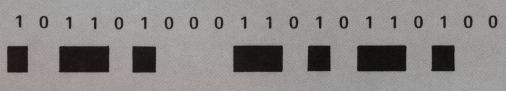
\includegraphics[width=10cm]{imgs/typical-config.png}}
% \caption{Nas renderizações, é convenção representar 1s como células em preto e 0s em branco. }
% \end{figure}

\tab Os ACEs são comumente representados por seu respectivo \textit{Wolfram code}, uma nomenclatura que dá a cada regra um identificador no intervalo \(\left[0, 255\right]\). Segundo \cite[p. 24]{wolfram2002new}, ``A linha superior em cada caixa dá uma das possíveis combinações de cores para uma célula e sua vizinhança imediata. A linha inferior então especifica qual será a cor da célula central no próximo passo em cada um desses casos.''

\begin{figure}[!htbp]
  \centerline{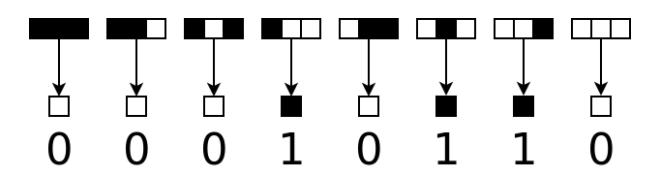
\includegraphics[width=10cm]{imgs/rule_22.png}}
  \caption{Ilustração do mapa de transições para a regra 22 no código Wolfram. }
\end{figure}

\begin{figure}[!htbp]
  \centerline{
\includegraphics[width=8cm]{imgs/256ecas.png}}
  \caption{Ilustração das 256 regras elementares. }
\end{figure}

% ACs de 1 dimensão, elementares, com vizinhança \texttt{\{-1,0,1\}}, com conjunto de estados \texttt{\{0,1\}}, na ordem lexicográfica \{\textit{\(w_0\)}, ..., \textit{\(w_7\)},\} em \(\{0,1\}^3\), se \(\delta(\textit{w}_i)=s_i,s_0,...s_7\) representa \(\delta\). Analogamente, qualquer inteiro positivo menor que 256 = \(2^8\) define um ACE \cite[cap. 2]{delorme1999introduction}.

% \begin{figure}[!htbp]
% \centerline{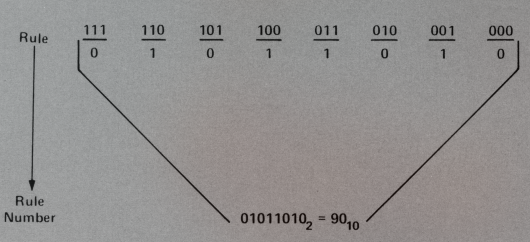
\includegraphics[width=10cm]{imgs/rule-transitions.png}}
% \caption{Ilustração do mapa de transições para a regra 90 na notação de \citeonline{wolfram1983cellular}}
% \end{figure}


% \cite{wolfram2002new}

% \tab ``O \textit{espaço celular} é um reticulado de n células idênticas, cada qual com um padrão idêntico de conexões locais para outras células e com condições de contorno. O conjunto de estados possíveis da célula é denotado por \(\Sigma\) e o número de estados desse conjunto é denotado por \textbf{k}. Cada célula é denotada por um índice \textbf{i} e seu estado a um dado tempo \textbf{t} é denotado por \(n_i^t\), onde \(S_i^t \in \Sigma\). O estado \(S_i^t\) da célula \textbf{i} e os estados das células às quais a célula \textbf{i} está conectada são chamados de vizinhança \(n_i^t\) da célula \textbf{i}.
%
% \tab A \textit{regra de transição} é denotada por \(\Phi(n_i^t)\) que fornece o próximo estado \(S_i^{t+1}\) para cada célula \textbf{i}, como uma função de \(n_i^t\). A cada passo de tempo, todas as células atualizam seus estados sincronicamente de acordo com \(\Phi(n_i^t)\). 

% \tab Para ACs unidimensionais, o tamanho da vizinhança \(n_i\) é normalmente escrito como \(\lvert n_i\rvert = 2r + 1\), onde \textbf{r} é chamado o raio do AC.''

% (como é descrito\ref{varia}).

\break
\subsubsection{ATUALIZAÇÃO ASSÍNCRONA \\POR PRIORIDADE DA VIZINHANÇA} \label{tiposatt}
\tab Parte imprescindível da definição de um AC é a ordem de atualização das células no espaço celular. Apesar de serem fundamentalmente concebidos com o comportamento de atualização síncrona, é possível se utilizar das mais diversas e criativas estratégias de atualização.

\tab No presente trabalho foi empregado um tipo inédito de estratégia de atualização: em função da prioridade da vizinhança, que consiste em cada uma das 8 regras de transição estar associada a uma prioridade no intervalo \(\left[1, 8\right]\), (e.g.: 12344321). Esse tipo de atualização requer uma distinção dos timesteps globais e locais (microtimesteps):  as prioridades de vizinhanças são iteradas sequencialmente de menor a maior e para cada prioridade, o espaço celular é varrido e atualizam-se apenas as células que tenham vizinhança com a prioridade atual, mantendo-se o estado das vizinhanças que não estejam na prioridade atual da iteração. Ao fim da varredura do espaço celular, o processo se repete para a próxima prioridade, agora iterando sobre o reticulado gerado no processo descrito anteriormente. O reticulado resultante após iterar sobre todas as prioridades é chamado de timestep global (ou macrotimestep) e é incluído nas renderizações, o que não acontece com os microtimesteps.

\tab Esse modo de atualização inclui também a atualização síncrona, que pode ser simulada quando as prioridades do esquema têm mesmo valor (11111111, 22222222, ..., etc). Diferentes esquemas de prioridade aplicados a uma mesma regra podem gerar evoluções idênticas. Estes esquemas são chamados esquemas equivalentes. As evoluções podem ser identificadas como um par \textit{(R,E)}, onde \textit{R} é a regra e \textit{E} é um esquema de prioridade. Eliminados os esquemas equivalentes, para ACEs, é possível gerar 1.194.165 combinações de pares \textit{(R,E)}. 

% \break 
\subsection{CONSERVABILIDADE NUMÉRICA} \label{num-conserv}
\tab Segundo \citeonline{boccara2002number}, ``Uma regra de AC \textit{f} de \textit{q} estados, unidimensional, de largura \textit{n} é conservativa se, para todas as configurações cíclicas de tamanho \textit{L} \(\geq\) n satisfaz'':

% ``A one-dimensional q-state n-input CA rule f is number-conserving if, for all cyclic configurations of length L \(\geq\) n, it satisfies'':

\[f(x_1,x_2,...,x_{n-1},x_n) + f(x_2,x_3,...,x_n,x_{n+1}) + ... \]
\tab \[ + \;   f(x_L,x_1,...,x_{n-2},x_{n-1} = x_1 + x_2 + ... + x_L\] 

% \break

\tab No contexto de ACEs, uma evolução é dita conservativa caso, para qualquer configuração inicial, a quantidade de um determinado estado é sempre a mesma para todos os timesteps. Como é mencionado no item \ref{contex}, ACs conservativos podem ser usados para modelar ambientes em que há conservabilidade, como trânsito automobilístico, simulação de partículas, entre outros. A regra 184 é uma regra que, com execução síncrona e (como este trabalho apresenta) assíncrona, gera evoluções conservativas pela definição anterior de conservabilidade.

\section{METODOLOGIA DA PESQUISA}
\tab No que tange à Metodologia empregada neste TCC, o trabalho teve início com uma revisão da literatura específica sobre o tema da pesquisa. Esta pesquisa abrange conceitos fundamentais de teoria da computação e o ``estado da arte'' em termos de análise de conservabilidade.

\tab Este alicerce teórico foi obtido através de autores como: Wolfram; Yuen e Kay; Boccara;
entre outros, além de pesquisas em periódicos científicos, sites, publicações em empresas, teses e dissertações em universidades e publicações de associações técnicas.  A leitura, análise e comparação da fundamentação teórica tiveram início com ACEs síncronos, modificados em seguida para viabilizar o tipo de atualização mencionado no item \ref{tiposatt}.

\subsection{ETAPAS DA PESQUISA}
\tab Para definir as etapas da pesquisa, foi necessário examinar as delimitações de estudo (item \ref{delimitacao}), desenvolvendo uma implementação que atendesse à execução dos ACE com esquemas totalmente distintos, como descrito no Cronograma apresentado no item \ref{cron}. No decorrer da fundamentação teórica foram realizados experimentos para verificação de conservabilidade inicialmente em modo de atualização síncrona e então assíncrona, com o objetivo de verificar conservabilidade. 

\tab Os 4683 esquemas de atualização mencionados no item \ref{objetopesq} foram testados primeiramente contra a regra 184, que é conservativa em modo síncrono. A extensão de evoluções celulares se limitou a N=15, como é explicitado no item \ref{delimitacao}.

% \break

Assim, pode-se dizer que as etapas desenvolvidas neste estudo foram:

\begin{enumerate}
  \item Revisão bibliográfica;
  \item Fundamentação teórica;
  \item Desenvolvimento e implementação em Python;
  \item Simulação;
  \item Análise das simulações;
  \item Conclusão e documentação final da pesquisa.
\end{enumerate}

\subsection{CLASSIFICAÇÃO DA PESQUISA}
\tab O tempo total previsto para a conclusão desta pesquisa é de 1 ano, como mostrado no capítulo \ref{cron}.

\tab Esta é uma pesquisa exploratória, dada a natureza desconhecida das propriedades de ACEs com o tipo de atualização mencionado em \ref{objetopesq}. Baseada em medidas objetivas e dados verificáveis, esta pesquisa foi voltada para encontrar caminhos, formas, maneiras e procedimentos para atingir um determinado fim, buscando definir um processo ou uma ferramenta que leve à solução do problema proposto.  Quanto aos meios, foram utilizados os recursos mencionados na Bibliografia.

\break

\section{CRONOGRAMA} \label{cron}

\tab As atividades desta pesquisa se desenvolveram de acordo com o cronograma apresentado a seguir, no prazo de 12 meses:

\newcommand{\ccy}{\cellcolor{yellow}}
\begin{table}[h]
  \caption{Cronograma de atividades}
  \centerline{
    \begin{tabular}{|l|l|l|l|l|l|l|l|l|l|l|l|l|} \hline
      \multirow{2}{*}{ATIVIDADE}                 & \multicolumn{12}{|c|}{MÊS} 							     \\
						 & 1    & 2    & 3    & 4    & 5    & 6    & 7    & 8    & 9    & 10   & 11   & 12   \\ \hline
      Revisão bibliográfica                      & \ccy & \ccy &      &      &      &      &      & \ccy &      &      &      &      \\ \hline
      Fundamentação teórica                      &      & \ccy & \ccy &      &      &      &      &      &      &      &      &      \\ \hline
      Desenvolvimento e implementação Python     &      & \ccy & \ccy &      &      &      &      &      &      &      &      &      \\ \hline
      Conclusão e documentação final da pesquisa &      &      &      & \ccy & \ccy &      &      &      &      &      &      &      \\ \hline
      Simulação                                  &      &      &      & \ccy & \ccy &      &      &      &      &      &      &      \\ \hline
      Análise das simulações                     &      &      &      &      &      & \ccy & \ccy &      &      &      &      &      \\ \hline
      Conclusão e documentação final da pesquisa &      &      &      &      &      & \ccy & \ccy & \ccy & \ccy & \ccy & \ccy & \ccy \\ \hline
    \end{tabular}
  }
\end{table}

% \break

\addcontentsline{toc}{section}{Referências}
\bibliography{cellz} \label{bib}

\end{document}
